\documentclass[11pt]{amsart}
\usepackage[T1]{fontenc}
\usepackage[utf8]{inputenc}
\usepackage{lmodern}
\usepackage[margin=1.15in]{geometry}
\usepackage{amsmath,amssymb,amsthm,mathtools}
\usepackage{booktabs}
\usepackage{microtype}
\usepackage{enumitem}
\usepackage{xcolor}
\usepackage{tikz}
\usepackage[hidelinks]{hyperref}
\usepackage{xurl}
\usepackage{orcidlink}
\usepackage[capitalise,nameinlink]{cleveref}

\newtheorem{theorem}{Theorem}[section]
\newtheorem{lemma}[theorem]{Lemma}
\newtheorem{corollary}[theorem]{Corollary}
\newtheorem{proposition}[theorem]{Proposition}
\theoremstyle{definition}
\newtheorem{definition}[theorem]{Definition}
\theoremstyle{remark}
\newtheorem{remark}[theorem]{Remark}

\newcommand{\fd}{f_{\delta\ge 3}}
\newcommand{\fc}{f_{\mathrm{cubic}}}
\newcommand{\Hseven}{H_7}
\newcommand{\Hfifteen}{H_{15}}
\newcommand{\Height}{H_8^{*}}
\newcommand{\lean}[1]{\texttt{#1}}

\usepackage{fancyvrb}
\DeclareUnicodeCharacter{2203}{\ensuremath{\exists}}
\DeclareUnicodeCharacter{2200}{\ensuremath{\forall}}
\DeclareUnicodeCharacter{2227}{\ensuremath{\wedge}}
\DeclareUnicodeCharacter{00AC}{\ensuremath{\neg}}
\DeclareUnicodeCharacter{2192}{\ensuremath{\to}}
\DeclareUnicodeCharacter{2264}{\ensuremath{\le}}
\DeclareUnicodeCharacter{27E8}{\ensuremath{\langle}}
\DeclareUnicodeCharacter{27E9}{\ensuremath{\rangle}}
\DefineVerbatimEnvironment{leancode}{Verbatim}{fontsize=\small,frame=single,framesep=2mm,rulecolor=\color{black!30}}

\title[Small graphs without power-of-two cycles]{Small graphs without cycles of length a power of two:\\ new bounds with kernel-checked proofs}

\author{Andrzej Marszałek\,\orcidlink{0009-0006-6148-2965}}
\address{Independent Researcher}
\urladdr{https://github.com/hipotures/conjectures}

\subjclass[2020]{05C38, 05C35, 68V15}
\keywords{Erdős–Gyárfás conjecture, cycle lengths, cubic graphs, vertex replacement, formal verification, Lean~4}

\date{27 November 2026}

\begin{document}

\begin{abstract}
The Erdős–Gyárfás conjecture states that every graph of minimum degree at least
three contains a cycle whose length is a power of two. Let $\fd(k)$ (respectively
$\fc(k)$) be the least order of a graph of minimum degree at least three
(respectively a cubic graph) with no cycle of length $4,8,\dots,2^k$. We prove
$\fd(4)\le 73$ and $\fd(5)\le 345$, using a new eight-vertex three-port gadget
$\Height$ together with the gadgets $\Hseven$ and $\Hfifteen$ of García. We also
show that, in Henry's oriented vertex-replacement construction, any set of
sources at pairwise distance at least nine may be replaced by seven-vertex
gadgets. Applied to Poláček's $702$-vertex cubic graph of girth $16$, with four
such sources, this gives $\fc(6)\le 10{,}498$. All of these statements,
including the girth of the $702$-vertex graph and Henry's bound
$\fc(5)\le 370$, are proved in a self-contained Lean~4 development that uses no
external libraries and no unverified code execution. An independent Python
program checks every construction.
\end{abstract}

\maketitle

%======================================================================
\section{Introduction}

A \emph{power-of-two cycle} is a cycle of length $2^j$ for some $j\ge 2$.

\begin{quote}
\textbf{Conjecture} (Erdős and Gyárfás, 1995; see~\cite{Erdos1997}).
Every finite simple graph of minimum degree at least three contains a
power-of-two cycle.
\end{quote}

The conjecture is open. It is known for graphs of large average
degree~\cite{LiuMontgomery2023} and in several structured classes, and
computer searches have excluded counterexamples of small order; for instance,
Ducoffe and Dumitru report that a counterexample has more than $40$
vertices~\cite{DucoffeDumitru2026}.

A natural way to measure how far small graphs are from being counterexamples
is to forbid only the first few power-of-two lengths. For $k\ge 2$ let
\begin{align*}
  \fd(k) &= \min\{\,|V(G)| : \delta(G)\ge 3,\ G \text{ has no cycle of length } 4,8,\dots,2^k\,\},\\
  \fc(k) &= \min\{\,|V(G)| : G \text{ is cubic and has no cycle of length } 4,8,\dots,2^k\,\}.
\end{align*}
Both functions are finite for every $k$: one replaces the vertices of a cubic
graph of large girth by small gadgets (\cref{sec:lifts}). The function $\fc$ is
the $f$ of García~\cite{Garcia2026} and Henry~\cite{Henry2026}, and
$\fd(k)\le\fc(k)$.

The Petersen graph gives $\fc(2)=10$, and the smallest cubic graphs without
cycles of length $4$ and $8$ have $24$ vertices~\cite{Markstrom2004,Garcia2026}.
Exoo~\cite{Exoo2014} constructed a cubic graph on $78$ vertices with no cycle
of length $4$, $8$ or $16$, and Ripatti's exhaustive search~\cite{Ripatti2017}
indicates that $\fc(4)=78$. For $k=5$, García~\cite{Garcia2026} gave a
corrected $450$-vertex construction, and Henry~\cite{Henry2026} lowered this to
$\fc(5)\le 370$. For $k=6$, García's general bound gives $\fc(6)\le 32{,}640$.
Henry proved $\fc(k)\le 15\,n_3(2^{k-2})-8$ for $k\ge 5$, where $n_3(g)$ is the
least order of a connected cubic graph of girth at least $g$, and noted that a
reported $702$-vertex cubic graph of girth $16$ would give $\fc(6)\le 10{,}522$.

\subsection*{Results}
\begin{theorem}\label{thm:main}
\leavevmode
\begin{enumerate}[label=\textup{(\roman*)}]
  \item $\fd(4)\le 73$;
  \item $\fd(5)\le 345$;
  \item $\fc(6)\le 10{,}498$.
\end{enumerate}
All witnesses are $2$-connected.
\end{theorem}

Parts (i) and (ii) use a new gadget $\Height$ on eight vertices with one vertex
of degree four (\cref{sec:gadgets}). The resulting graphs are smaller than the
best cubic constructions ($78$ and $370$ vertices). If Ripatti's search is
exhaustive, (i) shows that $\fd(4)<\fc(4)$. Part (iii) follows from a
\emph{source-packing} strengthening of Henry's one-source refinement
(\cref{thm:packing}), applied to Poláček's $702$-vertex cubic graph of girth
$16$ from the House of Graphs~\cite{HoG}. Henry did not have this graph; we
verify its girth formally.

\subsection*{Formal verification}
Each statement above is a theorem of a Lean~4~\cite{Lean4} library of about
$7{,}000$ lines. The library defines finite simple graphs and cycles from first
principles and proves the soundness of the cycle checkers it uses. All finite
computations, including a girth certificate for a $702$-vertex graph, are
performed by the Lean kernel itself. No \lean{native\_decide}, no external
solver and no axiom beyond Lean's three standard ones is used
(\cref{sec:formal}). The library also re-proves Henry's bound $\fc(5)\le 370$
and the existence of a $78$-vertex cubic graph without cycles of length $4$, $8$
and $16$.

\subsection*{Organisation}
\Cref{sec:lifts} recalls three-port vertex replacement and the cycle projection
lemma. \Cref{sec:gadgets} describes the gadgets. \Cref{sec:small} proves parts
(i) and (ii). \Cref{sec:packing} proves the source-packing theorem and part
(iii). \Cref{sec:formal} describes the formalization, and \cref{sec:repro}
explains how to reproduce the results.

%======================================================================
\section{Three-port vertex replacement}\label{sec:lifts}

All graphs are finite and simple. A \emph{three-port gadget} is a graph $H$
with three distinct \emph{ports} $p_0,p_1,p_2$ such that each port has degree
$2$ in $H$ and every other vertex has degree at least $3$. We write
$d_H(i,j)$ for the distance in $H$ between $p_i$ and $p_j$. It is also
convenient to allow the trivial gadget $U_1$, a single vertex that serves as all
three ports, with $d_{U_1}(i,j)=0$.

Let $B$ be a cubic graph. Suppose that at each vertex $v$ we are given a gadget
$H_v$ and a bijection $\sigma_v$ from the three edges at $v$ to the port indices
$\{0,1,2\}$. The \emph{lift} $B[H,\sigma]$ is obtained from the disjoint union
of the $H_v$ by adding, for every edge $uv$ of $B$, an edge between port
$\sigma_u(uv)$ of $H_u$ and port $\sigma_v(uv)$ of $H_v$. Every vertex of the
lift then has degree at least $3$, and the lift is cubic when every non-port
vertex of every gadget has degree exactly $3$. Its order is
$\sum_v |V(H_v)|$.

For a cycle $D=(v_1,\dots,v_\ell)$ of $B$ and a vertex $v_i$ of $D$, let
$a_i=\sigma_{v_i}(v_{i-1}v_i)$ and $b_i=\sigma_{v_i}(v_iv_{i+1})$ (indices
modulo $\ell$), and define the \emph{weight}
\[
  w(D)=\sum_{i=1}^{\ell}\bigl(1+d_{H_{v_i}}(a_i,b_i)\bigr).
\]

\begin{lemma}[Cycle projection; cf.~\cite{Garcia2026,Henry2026}]\label{lem:projection}
Every cycle $C$ of $B[H,\sigma]$ either lies inside a single gadget $H_v$, or
there is a cycle $D$ of $B$ with $|C|\ge w(D)$.
\end{lemma}

\begin{proof}[Sketch]
Suppose $C$ meets at least two gadgets. Contract every gadget to its base
vertex. Each maximal run of $C$ inside a gadget $H_v$ enters and leaves through
two different ports. A non-trivial gadget has only three ports, so $C$ visits
it in exactly one run; for $U_1$ this holds because $C$ is simple. Hence the
contracted closed walk is a cycle $D$ of $B$. The run inside $H_{v_i}$ is a
path between ports $a_i$ and $b_i$, so it has at least $d_{H_{v_i}}(a_i,b_i)$
edges. Adding the $\ell$ edges between gadgets gives $|C|\ge w(D)$.
\end{proof}

The formal version (\lean{liftGraph\_cycle\_dichotomy}) also shows that $D$
has length at least $3$ and that, in the first case, $C$ is a cycle of $H_v$.
We use the lemma in the following form.

\begin{corollary}\label{cor:criterion}
Let $L\ge 3$. Suppose no gadget $H_v$ contains a cycle of length $L$ and
$w(D)>L$ for every cycle $D$ of $B$. Then $B[H,\sigma]$ has no cycle of
length $L$.
\end{corollary}

In our constructions $\sigma_v$ is determined by one distinguished neighbour
$q(v)$ of $v$: the edge $vq(v)$ goes to port $0$, and the other two edges go to
ports $1$ and $2$. For the gadgets below, $d_H(0,1)=d_H(0,2)$, so $w(D)$
depends only on the map $q$ and on the gadget at each vertex. (The exact rule
for ports $1$ and $2$, which fixes the graph up to isomorphism, is given with
the data in \cref{sec:repro}.)

%======================================================================
\section{Gadgets}\label{sec:gadgets}

\begin{table}[ht]
\centering
\caption{The gadgets. $d(0,\cdot)$ is the common value of $d(0,1)=d(0,2)$.
Cycle lengths were found by exhaustive enumeration. None of the gadgets
contains a cycle of length $4$ or $8$, and all have fewer than $16$ vertices.}
\label{tab:gadgets}
\begin{tabular}{@{}lcccll@{}}
\toprule
Gadget & order & $d(0,\cdot)$ & $d(1,2)$ & degrees & internal cycle lengths\\
\midrule
$\Hseven$ \cite{Garcia2026}   & 7  & 2 & 3 & $2^3\,3^4$ & 3, 5, 6, 7\\
$\Height$ (new)               & 8  & 3 & 2 & $2^3\,3^4\,4^1$ & 3, 5, 6, 7\\
$\Hfifteen$ \cite{Garcia2026} & 15 & 3 & 5 & $2^3\,3^{12}$ & 3, 5, 6, 7, 9--15\\
$U_1$                         & 1  & 0 & 0 & -- & none\\
\bottomrule
\end{tabular}
\end{table}

We use the following labelled versions. Ports are listed as $(p_0,p_1,p_2)$.
\begin{itemize}[leftmargin=1.5em]
\item $\Hseven$: vertices $0,\dots,6$; edges
  $03,04,13,15,24,26,35,46,56$; ports $(0,1,2)$.
\item $\Hfifteen$: two copies of $\Hseven$ on $\{0,\dots,6\}$ and
  $\{7,\dots,13\}$, a new vertex $14$, and edges $14\text{--}1$,
  $14\text{--}8$, $2\text{--}9$; ports $(14,0,7)$. Up to relabelling this is
  García's $\Hfifteen$; its cycle spectrum agrees with~\cite[Table~2]{Henry2026}.
\item $\Height$: vertices $0,\dots,7$; edges
  $03,04,13,16,25,27,35,46,47,57,67$; ports $(2,0,1)$. Vertex $7$ has degree
  $4$.
\end{itemize}

\begin{figure}[ht]
\centering
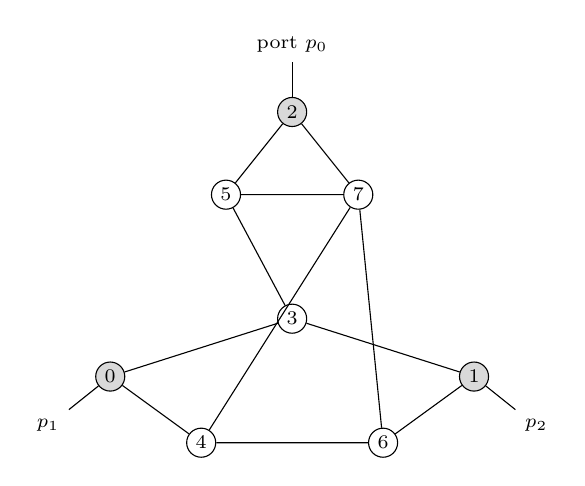
\begin{tikzpicture}[scale=1.05,
  v/.style={circle,draw,fill=white,inner sep=1.6pt,font=\scriptsize},
  p/.style={circle,draw,fill=black!15,inner sep=1.6pt,font=\scriptsize}]
  \node[p] (2) at (0,2.3) {2};
  \node[p] (0) at (-2.2,-0.9) {0};
  \node[p] (1) at (2.2,-0.9) {1};
  \node[v] (5) at (-0.8,1.3) {5};
  \node[v] (7) at (0.8,1.3) {7};
  \node[v] (3) at (0,-0.2) {3};
  \node[v] (4) at (-1.1,-1.7) {4};
  \node[v] (6) at (1.1,-1.7) {6};
  \foreach \a/\b in {0/3,0/4,1/3,1/6,2/5,2/7,3/5,4/6,4/7,5/7,6/7}
    \draw (\a)--(\b);
  \draw (2)--++(0,0.6) node[above,font=\scriptsize]{port $p_0$};
  \draw (0)--++(-0.5,-0.4) node[below left,font=\scriptsize]{$p_1$};
  \draw (1)--++(0.5,-0.4) node[below right,font=\scriptsize]{$p_2$};
\end{tikzpicture}
\caption{The gadget $\Height$. Ports are shaded; the edge stubs show where the
gadget is attached to the base graph. Vertex $7$ has degree $4$.}
\label{fig:h8}
\end{figure}

Compared with $\Hseven$, the gadget $\Height$ has one more vertex, but its
distinguished port $p_0$ is at distance $3$ from the other two ports. In a lift,
a cycle that passes through an $\Height$ via $p_0$ therefore gains one edge
over an $\Hseven$, and one that avoids $p_0$ loses one. This trade-off is what
yields the two bounds in \cref{sec:small}.

The port distances are certified in Lean by explicit potentials: functions
$\varphi\colon V(H)\to\mathbb{N}$ with $\varphi(p_i)=0$ that increase by at most
one along each edge, so $\varphi(x)\le d_H(p_i,x)$. The absence of $4$- and
$8$-cycles is certified by a cycle search whose soundness is proved in Lean.

%======================================================================
\section{Small graphs: proofs of parts (i) and (ii)}\label{sec:small}

\subsection{Seventy-three vertices}
Let $B$ be the Petersen graph with vertices $0,\dots,9$ and neighbourhoods
\[
\begin{array}{c|cccccccccc}
v & 0&1&2&3&4&5&6&7&8&9\\\hline
N(v) & 1,4,5 & 0,2,6 & 1,3,7 & 2,4,8 & 0,3,9 & 0,7,8 & 1,8,9 & 2,5,9 & 3,5,6 & 4,6,7
\end{array}
\]
Put $\Height$ at the vertices $0,1,2$ and $\Hseven$ at the other seven vertices,
with distinguished neighbours
\[
(q(0),\dots,q(9))=(1,6,1,2,0,0,1,2,6,6).
\]
(The construction was found by a computer search over gadget assignments and
the maps $q$.)
The lift has $3\cdot 8+7\cdot 7=73$ vertices and $111$ edges, $70$ vertices of
degree $3$ and $3$ of degree $4$.

\begin{proof}[Proof of \cref{thm:main}(i)]
The Petersen graph has $57$ cycles: $12$, $10$, $15$ and $20$ of lengths
$5,6,8,9$. A direct computation shows $w(D)\ge 17$ for each of them (the minimum
is attained). No gadget contains a cycle of length $4$, $8$ or $16$
(\cref{tab:gadgets}). By \cref{cor:criterion} the lift has no cycle of length
$4$, $8$ or $16$.
\end{proof}

A second, structurally different witness keeps vertex $0$ of the Petersen graph
as $U_1$ and puts $\Height$ at the other nine vertices, with
$q=(1,0,1,4,0,0,1,5,5,4)$. It also has $73$ vertices; it has $114$ edges and
nine vertices of degree $4$. Both witnesses are $2$-connected. We do not know
whether $\fd(4)<73$.

\subsection{Three hundred and forty-five vertices}
Let $B$ be the Tutte--Coxeter graph~\cite{Tutte1947}, the $(3,8)$-cage on $30$
vertices, labelled as in \cref{tab:tc}. Put $\Hfifteen$ at the fifteen vertices
\[
0,1,2,5,7,8,14,15,16,18,21,22,25,28,29
\]
and $\Height$ at the other fifteen, with the distinguished neighbours $q$ of
\cref{tab:tc}. The lift has $15\cdot 15+15\cdot 8=345$ vertices.

\begin{proof}[Proof of \cref{thm:main}(ii)]
Every vertex of $B$ contributes at least $1+2=3$ to the weight of a cycle
through it, so $w(D)\ge 3|D|\ge 33$ whenever $|D|\ge 11$. The Tutte--Coxeter
graph is bipartite of girth $8$, so it remains to check its $90$ cycles of
length $8$ and $72$ cycles of length $10$. A direct computation gives $w(D)\ge 33$
for all $162$ of them. Hence $w(D)>32$ for every cycle $D$ of $B$. No gadget
contains a cycle of length $4$, $8$, $16$ or $32$. By \cref{cor:criterion} the
lift has no cycle of length $4,8,16,32$.
\end{proof}

\begin{table}[ht]
\centering
\caption{Tutte--Coxeter graph: neighbourhoods $N(v)$, and the distinguished
neighbours $q(v)$ for the $345$-vertex lift ($q_{345}$) and for the $370$-vertex
lift ($q_{370}$).}
\label{tab:tc}
\footnotesize
\begin{tabular}{@{}r@{\;}c@{\;}c@{\;}c@{\qquad}r@{\;}c@{\;}c@{\;}c@{\qquad}r@{\;}c@{\;}c@{\;}c@{}}
\toprule
$v$ & $N(v)$ & $q_{345}$ & $q_{370}$ & $v$ & $N(v)$ & $q_{345}$ & $q_{370}$ & $v$ & $N(v)$ & $q_{345}$ & $q_{370}$\\
\midrule
0 & 1,17,29 & 29 & 29 & 10 & 9,11,19 & 11 & 19 & 20 & 19,21,27 & 19 & 19\\
1 & 0,2,22 & 0 & 0 & 11 & 10,12,24 & 12 & 24 & 21 & 14,20,22 & 22 & 20\\
2 & 1,3,9 & 1 & 3 & 12 & 11,13,29 & 13 & 13 & 22 & 1,21,23 & 1 & 23\\
3 & 2,4,26 & 26 & 26 & 13 & 4,12,14 & 4 & 14 & 23 & 6,22,24 & 24 & 6\\
4 & 3,5,13 & 3 & 13 & 14 & 13,15,21 & 21 & 21 & 24 & 11,23,25 & 11 & 23\\
5 & 4,6,18 & 18 & 6 & 15 & 8,14,16 & 14 & 14 & 25 & 16,24,26 & 16 & 24\\
6 & 5,7,23 & 23 & 7 & 16 & 15,17,25 & 15 & 25 & 26 & 3,25,27 & 27 & 25\\
7 & 6,8,28 & 8 & 8 & 17 & 0,16,18 & 18 & 0 & 27 & 20,26,28 & 20 & 20\\
8 & 7,9,15 & 15 & 9 & 18 & 5,17,19 & 17 & 17 & 28 & 7,27,29 & 7 & 7\\
9 & 2,8,10 & 10 & 2 & 19 & 10,18,20 & 10 & 18 & 29 & 0,12,28 & 28 & 12\\
\bottomrule
\end{tabular}
\end{table}

\begin{remark}[Henry's $370$-vertex graph]
With $\Hseven$ at the ten vertices $1,4,5,10,11,15,16,22,27,28$ of
\cref{tab:tc}, $\Hfifteen$ elsewhere, and the column $q_{370}$, the same
argument (minimum weight $33$ over the $162$ short cycles) gives a cubic graph
on $370$ vertices with no cycle of length $4,8,16,32$. We found this
construction independently, but Henry~\cite{Henry2026} published the bound
$\fc(5)\le 370$ first, with a construction of the same type. Our contribution
here is a formal proof.
\end{remark}

%======================================================================
\section{Source packings and $\fc(6)$}\label{sec:packing}

Let $B$ be a cubic graph and let $f\colon V(B)\to V(B)$ map each vertex to one
of its neighbours. We call $f$ an \emph{orientation}, and a vertex $s$ a
\emph{source} if $f(v)\ne s$ for every $v$. A \emph{directed cycle of length
$t$} is a vertex $x$ with $f^t(x)=x$.

\begin{theorem}[Source packing]\label{thm:packing}
Let $B$ be a cubic graph on $N$ vertices of girth at least $16$, and let $f$ be
an orientation of $B$ without directed cycles of length $1,\dots,16$. Let $S$ be
a set of sources of $f$ that are pairwise at distance at least $9$ in $B$. Put
$\Hseven$ at the vertices of $S$ and $\Hfifteen$ at all other vertices, with
distinguished neighbour $q(v)=f(v)$. The lift is a cubic graph on $15N-8|S|$
vertices with no cycle of length $4,8,16,32$ or $64$.
\end{theorem}

Henry's refinement~\cite[Theorem~5.2]{Henry2026} is essentially the case
$|S|=1$, for an orientation that he builds explicitly. \Cref{thm:packing}
separates the properties that the argument uses: no short directed cycles, and
sources far apart.

\begin{proof}
Both gadgets are cubic apart from their ports, so the lift is cubic. Its order
is $7|S|+15(N-|S|)=15N-8|S|$. Neither gadget contains a power-of-two cycle
(\cref{tab:gadgets}). Let $D=(v_1,\dots,v_\ell)$ be a cycle of $B$, so
$\ell\ge 16$. The contribution $1+d(a_i,b_i)$ of $v_i$ to $w(D)$ is
\begin{itemize}[leftmargin=1.5em]
\item at least $3$ if $v_i\in S$;
\item at least $4$ if $v_i\notin S$, and equal to $6$ if moreover
  $f(v_i)\notin\{v_{i-1},v_{i+1}\}$, because then $D$ passes $\Hfifteen$
  through ports $1$ and $2$.
\end{itemize}
In particular $w(D)\ge 3\ell\ge 48>32$, which excludes lengths $4,8,16,32$ by
\cref{cor:criterion}. It remains to show $w(D)\ge 65$.

Two sources on $D$ are at distance at least $9$ in $B$, so at least $9$ along
$D$. Hence $|D\cap S|\le\lfloor \ell/9\rfloor$. If $\ell\ge 17$, then
$w(D)\ge 4\ell-\lfloor\ell/9\rfloor\ge 68-1=67$, because the left-hand side is
increasing in $\ell$.

Let $\ell=16$, so $|D\cap S|\le 1$. We claim that some $v\in D\setminus S$
satisfies $f(v)\notin\{v^-,v^+\}$, where $v^\pm$ are its neighbours on $D$.
Otherwise $f$ maps $D\setminus S$ into $V(D)$, and no vertex maps to a source.
So $f$ maps the nonempty set $D\setminus S$ into itself. Iterating $f$ on this
set, which has at most $16$ elements, produces a directed cycle of length at
most $16$, a contradiction. That vertex contributes $6$ instead of $4$, so
$w(D)\ge 4\cdot 16-1+2=65$.
\end{proof}

\begin{proof}[Proof of \cref{thm:main}(iii)]
Let $B$ be Poláček's cubic graph on $702$ vertices (House of
Graphs~\cite{HoG}, file \texttt{k3\_g16\_n702.g6}, SHA-256 prefix
\texttt{b94c67a6}). It is bipartite with girth $16$. We fix an orientation $f$
without directed cycles of length at most $16$, and four of its sources,
\[
S=\{10,\,296,\,402,\,469\},
\]
pairwise at distance at least $9$. The orientation is listed in the repository
(\cref{sec:repro}); only the stated properties are used, and they are checked
both in Lean and by the independent checker. \Cref{thm:packing} gives a cubic
graph on $15\cdot 702-8\cdot 4=10{,}498$ vertices with no cycle of length
$4,8,16,32,64$.
\end{proof}

\begin{remark}
The girth of $B$ is the delicate input: Henry's bound $10{,}522$ was
conditional on the existence of this graph, which he did not reconstruct. In the
formal proof the girth is established as follows. Two explicit permutations of
$V(B)$ are checked to be automorphisms, and the group they generate is checked
to act transitively on one colour class of the bipartition. A breadth-first
search tree of depth $7$ from a fixed vertex of that class certifies that no
cycle of length less than $16$ passes through it. Every cycle meets both colour
classes, so it can be moved by an automorphism to pass through the fixed
vertex. Hence $B$ has girth at least $16$.
\end{remark}

\begin{remark}
We used only $|S|=4$; a larger packing of sources would improve the bound. The
library also contains a variant for bases of girth at least $17$, where the vertices of a greedily chosen maximal $4$-packing (pairwise
distance at least $5$) receive $\Hseven$, without using an orientation
(\lean{f\_cubic\_6\_4packing}). With the known
$2048$-vertex cubic graph of girth $17$ it gives a weaker bound.
\end{remark}

%======================================================================
\section{The formalization}\label{sec:formal}

The Lean library \lean{ErdosGyarfas} depends only on the Lean~4 core library
(version 4.36.0). Graphs are defined from first principles:

\begin{leancode}
structure FinGraph (n : Nat) where
  adj : Fin n → Fin n → Bool
  symm : ∀ u v : Fin n, adj u v = adj v u
  loopless : ∀ u : Fin n, adj u u = false

structure SimpleCycle (G : FinGraph n) (L : Nat) where
  hlen : 3 ≤ L
  vert : Fin L → Fin n
  inj : ∀ i j : Fin L, vert i = vert j → i = j
  edge : ∀ i : Fin L,
    G.adj (vert i) (vert ⟨(i.val + 1) % L, _⟩) = true

def HasCycle (G : FinGraph n) (L : Nat) : Prop := Nonempty (SimpleCycle G L)
\end{leancode}

Degrees count neighbours, \lean{IsCubic} means that every degree is $3$, and
\lean{MinDegAtLeast 3} that every degree is at least $3$. With these
definitions the three parts of \cref{thm:main} read:

\begin{leancode}
theorem f_delta3_4_le_73 : ∃ G : FinGraph 73,
    G.MinDegAtLeast 3 ∧ ¬ G.HasCycle 4 ∧ ¬ G.HasCycle 8 ∧ ¬ G.HasCycle 16

theorem f_delta3_5_le_345 : ∃ G : FinGraph 345,
    G.MinDegAtLeast 3 ∧ ¬ G.HasCycle 4 ∧ ¬ G.HasCycle 8 ∧
    ¬ G.HasCycle 16 ∧ ¬ G.HasCycle 32

theorem f_cubic_6_le_10498 : ∃ G : FinGraph 10498,
    G.IsCubic ∧ ¬ G.HasCycle 4 ∧ ¬ G.HasCycle 8 ∧ ¬ G.HasCycle 16 ∧
    ¬ G.HasCycle 32 ∧ ¬ G.HasCycle 64
\end{leancode}

The proofs follow the paper. \Cref{lem:projection} is proved once for arbitrary
bases and gadgets (\lean{liftGraph\_cycle\_dichotomy}), and so is
\cref{thm:packing} (\lean{f\_cubic\_6\_source\_8packing}). The finite facts are
then checked by kernel reduction. These are the weights $w(D)$ over all short
base cycles, the gadget properties, the automorphisms and the search tree for
the $702$-vertex graph, the absence of short directed cycles of $f$, and the
distances between the sources. Each check is a Boolean function together with
a Lean proof that a \lean{true} result implies the mathematical property. Lean
evaluates the function with \lean{decide} or \lean{rfl}, so the kernel itself
performs the computation. Large data, such as the $702$-vertex adjacency table,
are stored as balanced $4$-ary trees so that lookups stay cheap during kernel
reduction.

We do not use \lean{native\_decide}. That tactic trusts compiled code and adds
the axiom \lean{Lean.ofReduceBool}. For every headline theorem,
\lean{\#print axioms} reports at most \lean{propext}, \lean{Classical.choice}
and \lean{Quot.sound}. A continuous-integration job rebuilds the library on
every change. It fails if any reported axiom is outside this set, or if
\lean{sorry}, \lean{native\_decide}, \lean{implemented\_by}, \lean{extern} or an
\lean{axiom} declaration appears in the code. A full build takes about one
minute on a desktop computer.

The library also proves that every witness is $2$-connected. This is shown for
lifts in general (\lean{liftGraph\_is2Connected}) and checked on the bases and
gadgets. It also contains two results that are not part of this paper:
double-counting bounds for lifts of the Tutte--Coxeter graph, and reductions for
cubic bipartite graphs, which support computer-assisted lower bounds to be
reported separately.

%======================================================================
\section{Reproducibility}\label{sec:repro}

Everything is available at \url{https://github.com/hipotures/conjectures}, in
the folder \texttt{results/small-graphs-power-of-two-cycles}. It contains:
\begin{itemize}[leftmargin=1.5em]
\item the Lean library and an axiom audit (\texttt{lake build} and
  \texttt{scripts/check\_axioms.py});
\item \texttt{data/constructions.json}, extracted mechanically from the Lean
  sources: gadgets, bases, gadget assignments and orientations. At a base vertex
  $v$ with neighbour list $(n_0,n_1,n_2)$ as in the tables above and
  $q(v)=n_c$, the neighbour $n_k$ is attached to port $(k-c)\bmod 3$;
\item graph6 files of the $73$-, $345$- and $370$-vertex witnesses, and the
  House of Graphs file of the $702$-vertex base;
\item \texttt{verify.py}, an independent checker in plain Python without
  dependencies.
\end{itemize}

The checker rebuilds every lift from the data and confirms the orders, degrees
and $2$-connectivity. It recomputes the port distances and cycle spectra of the
gadgets by brute force. It confirms by exhaustive search that the
$73$-vertex graphs and the $78$-vertex cubic graph have no cycle of length
$4$, $8$ or $16$, and that the $345$- and $370$-vertex graphs have no cycle of
length $4$, $8$ or $16$; the absence of $32$-cycles is covered by the weight
computation. It recomputes $w(D)$ over all relevant base cycles. For
the $702$-vertex base it checks the girth by breadth-first search, the
orientation, the sources, and $w(D)\ge 65$ for every $16$-cycle. Its code shares
nothing with the Lean development except the input data.

\section*{Use of AI tools}
This work was carried out with substantial assistance from AI systems, mainly
Gemini~4~Neon (Google) and Claude Opus~5.5 (Anthropic), used through the
Antigravity and Claude Code environments. They were used to search for
constructions, write the Lean development and the checking code, and draft the
text. AI systems are not authors of this paper. All mathematical claims are
checked by the Lean kernel as described in \cref{sec:formal}, and the author
takes responsibility for the content and for the attribution of prior work.

\section*{Acknowledgements}
We thank the maintainers of the House of Graphs for making the $702$-vertex
graph available.

\begin{thebibliography}{99}

\bibitem{Erdos1997}
P.~Erdős, \emph{Some old and new problems in various branches of combinatorics},
Discrete Math. \textbf{165/166} (1997), 227--231.

\bibitem{DucoffeDumitru2026}
G.~Ducoffe and A.~Dumitru, \emph{Towards a more structured search for
Erdős--Gyárfás counterexamples}, arXiv:2609.28594, 2026.

\bibitem{Exoo2014}
G.~Exoo, \emph{Three graphs and the Erdős--Gyárfás conjecture},
arXiv:1403.5636, 2014.

\bibitem{EGJSV2026}
G.~Exoo, J.~Goedgebeur, J.~Jooken, L.~Stubbe and T.~Van den Eede,
\emph{New small regular graphs of given girth: the cage problem and beyond},
Electron. J. Combin. \textbf{33}(3) (2026), \#P3.48.

\bibitem{Garcia2026}
D.~García, \emph{Small graphs without power-of-two cycles: a lower bound of 24,
a correction to a construction of Exoo, and explicit bounds for $f(k)$},
arXiv:2609.04686, 2026.

\bibitem{Henry2026}
K.~Henry, \emph{Improved cubic graph constructions avoiding power-of-two cycle
lengths}, preprint, Zenodo, 2026, \url{https://doi.org/10.5281/zenodo.23886386}.

\bibitem{HoG}
K.~Coolsaet, S.~D'hondt and J.~Goedgebeur, \emph{House of Graphs 2.0: a
database of interesting graphs and more}, Discrete Appl. Math. \textbf{325}
(2023), 97--107. Cage data: \url{https://houseofgraphs.org/meta-directory/cages}.

\bibitem{Lean4}
L.~de Moura and S.~Ullrich, \emph{The Lean 4 theorem prover and programming
language}, in: Automated Deduction -- CADE 28, Lecture Notes in Comput. Sci.
\textbf{12699}, Springer, 2021, 625--635.

\bibitem{LiuMontgomery2023}
H.~Liu and R.~Montgomery, \emph{A solution to Erdős and Hajnal's odd cycle
problem}, J. Amer. Math. Soc. \textbf{36} (2023), 1191--1234.

\bibitem{Markstrom2004}
K.~Markström, \emph{Extremal graphs for some problems on cycles in graphs},
Congr. Numer. \textbf{171} (2004), 179--192.

\bibitem{Ripatti2017}
A.~V.~Ripatti, \emph{Faster approach for exhaustive search over graphs with
certain properties}, abstract, BAIKAL 2017 conference, 2017.

\bibitem{Tutte1947}
W.~T.~Tutte, \emph{A family of cubical graphs}, Proc. Cambridge Philos. Soc.
\textbf{43} (1947), 459--474.

\end{thebibliography}

\end{document}
